\subsection{External Interface Requirements}

\subsubsection{User Interfaces}
\begin{figure}
[H]
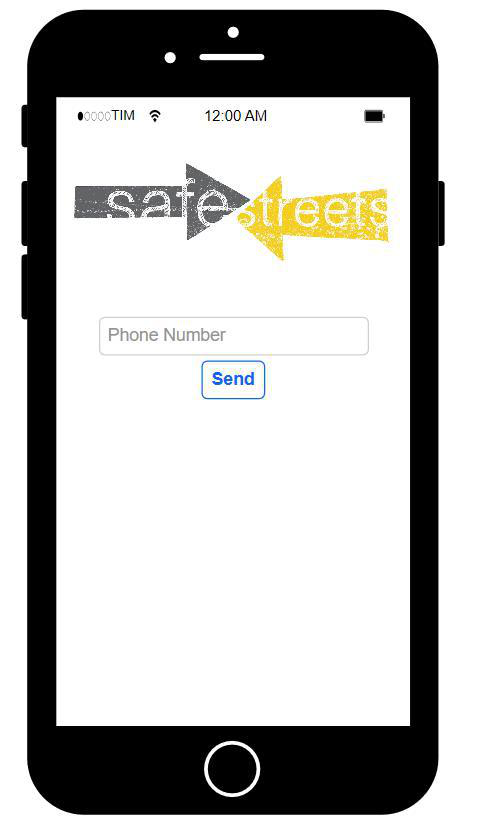
\includegraphics[scale=0.52]{Images/Templates/User/us_0.png}
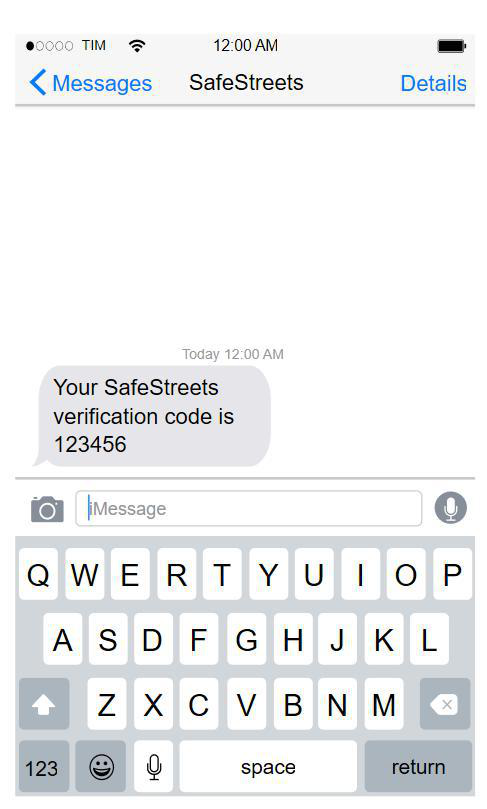
\includegraphics[scale=0.5]{Images/Templates/User/us_1.png}
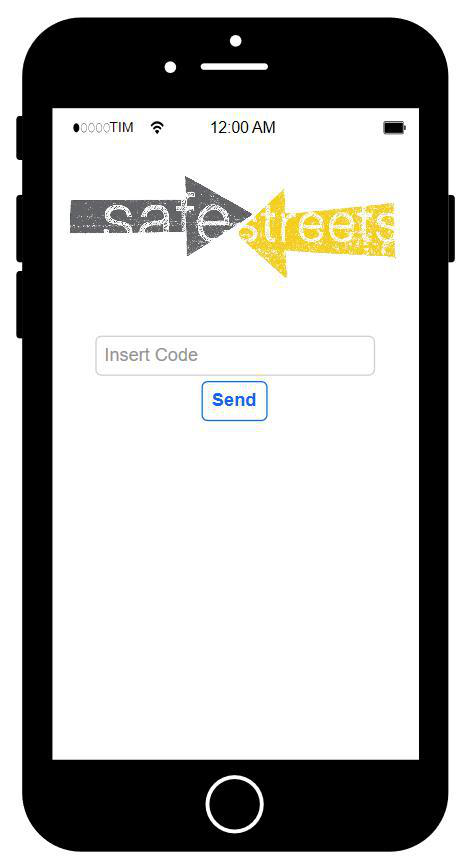
\includegraphics[scale=0.5]{Images/Templates/User/us_2.png}
\caption{\label{fig:Mockup-1}Login}
\end{figure}

This is the first page the users are shown. To continue they have to input their cellphone number and to insert an OTP sent to them by the system.

\begin{figure} [H]
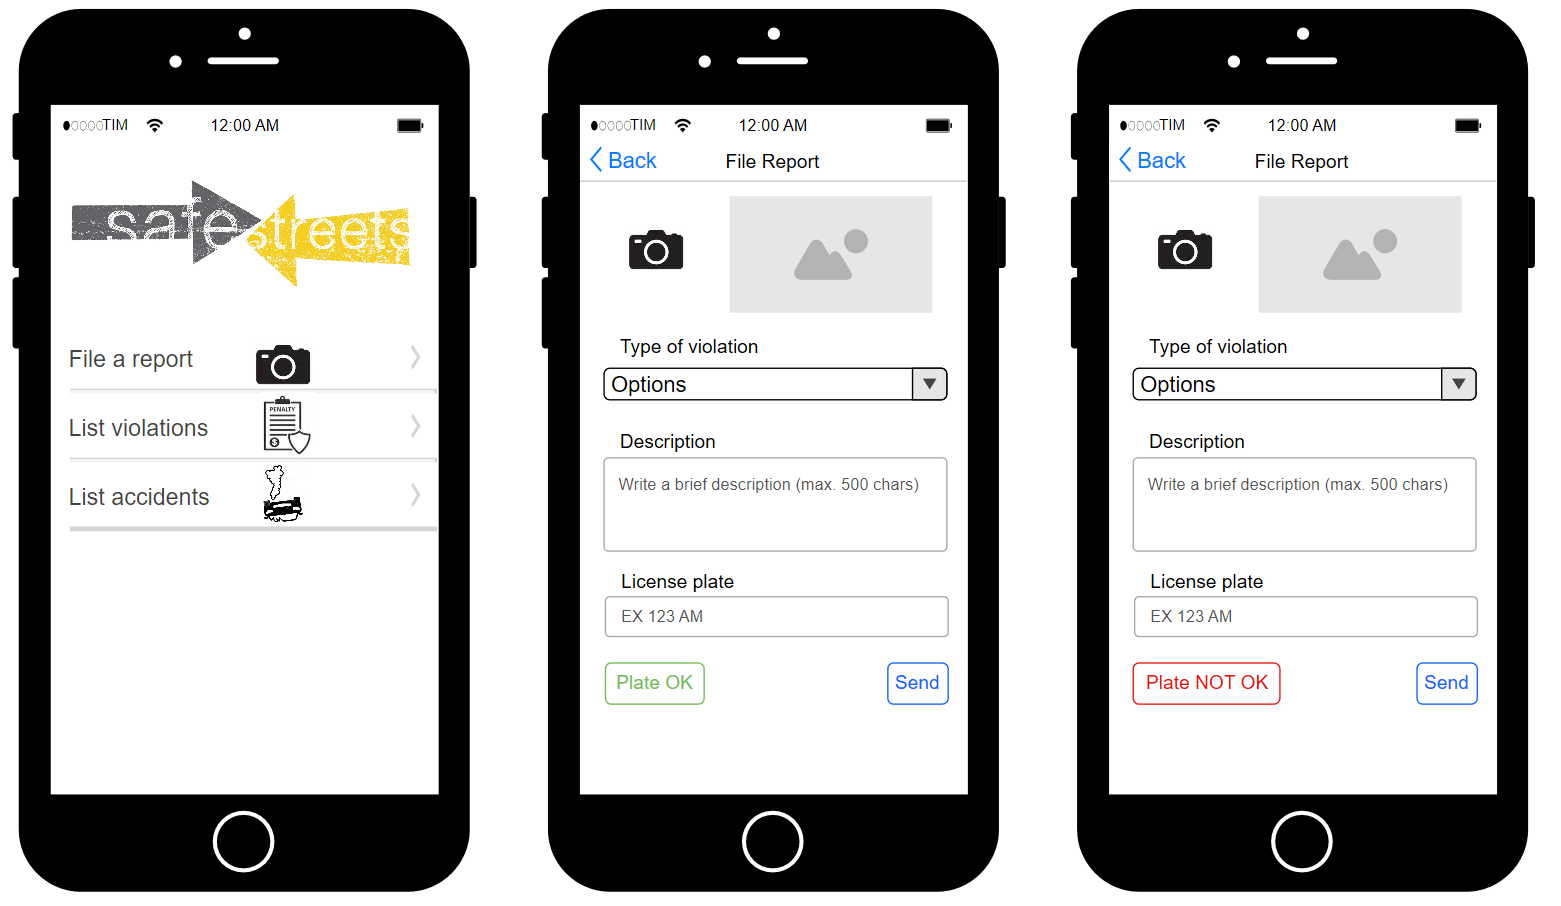
\includegraphics[scale=0.47]{Images/Templates/User/us_3.PNG}
\caption{\label{fig:Mockup-2}Menu and File Report section}
In this case it is shown how the report of violations is handled. The users enters the correct area and fills all the fields. If the plate is recognized, the report can be sent. This does not happen in the opposite case.
\end{figure}


\begin{figure}[t]
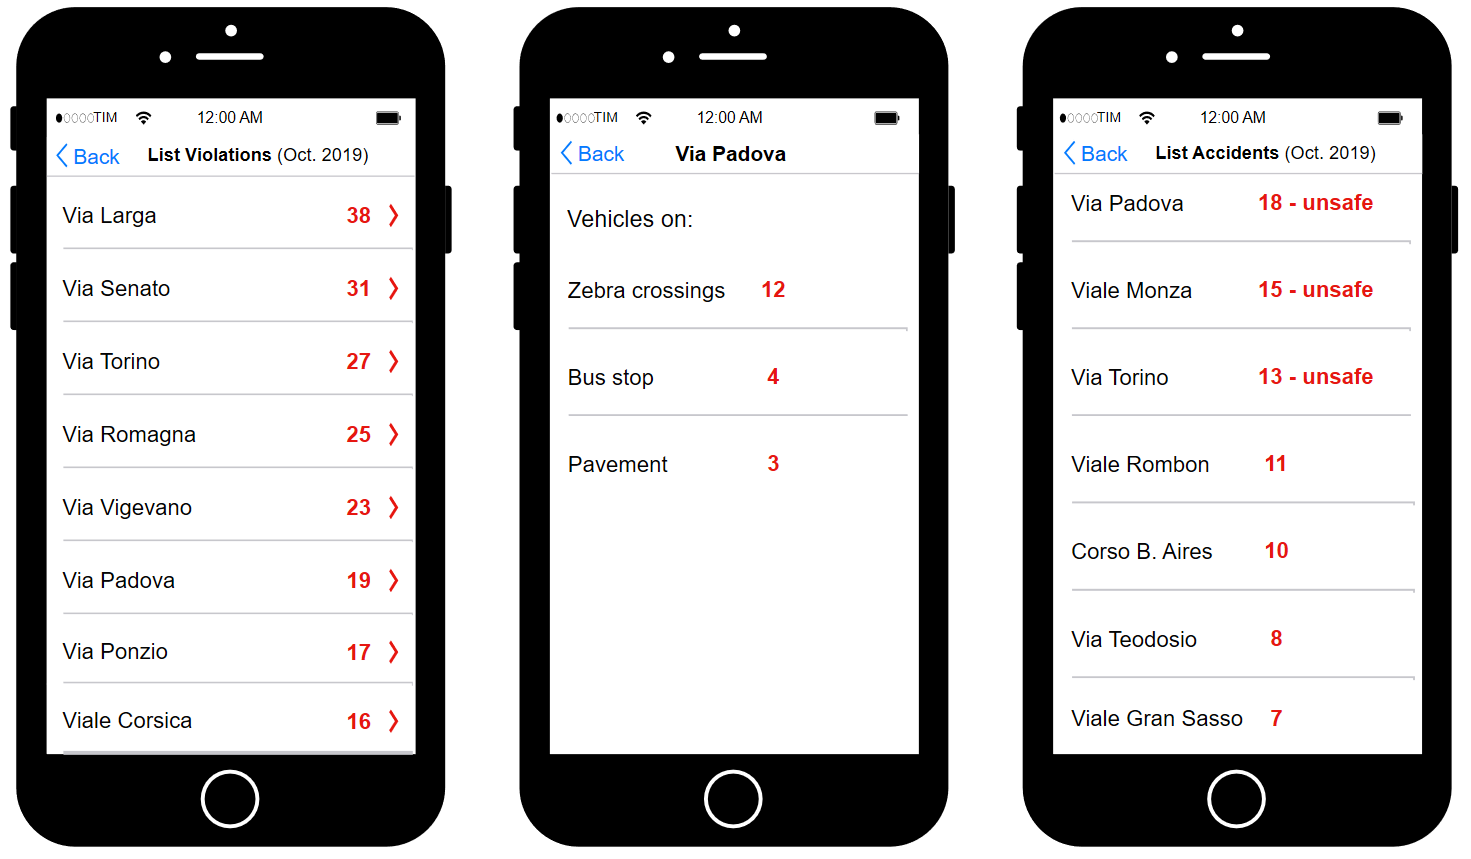
\includegraphics[scale=0.5]{Images/Templates/User/us_4.PNG}
\caption{\label{fig:Mockup-3}List Violations and List Accidents sections}
Upon entering on the apposite areas, the users are shown a list of streets with information about violations. If a precise one is selected, the types are linked to their quantities.
\end{figure}


\subsubsection{Authority Interfaces}
\begin{figure}
[H]
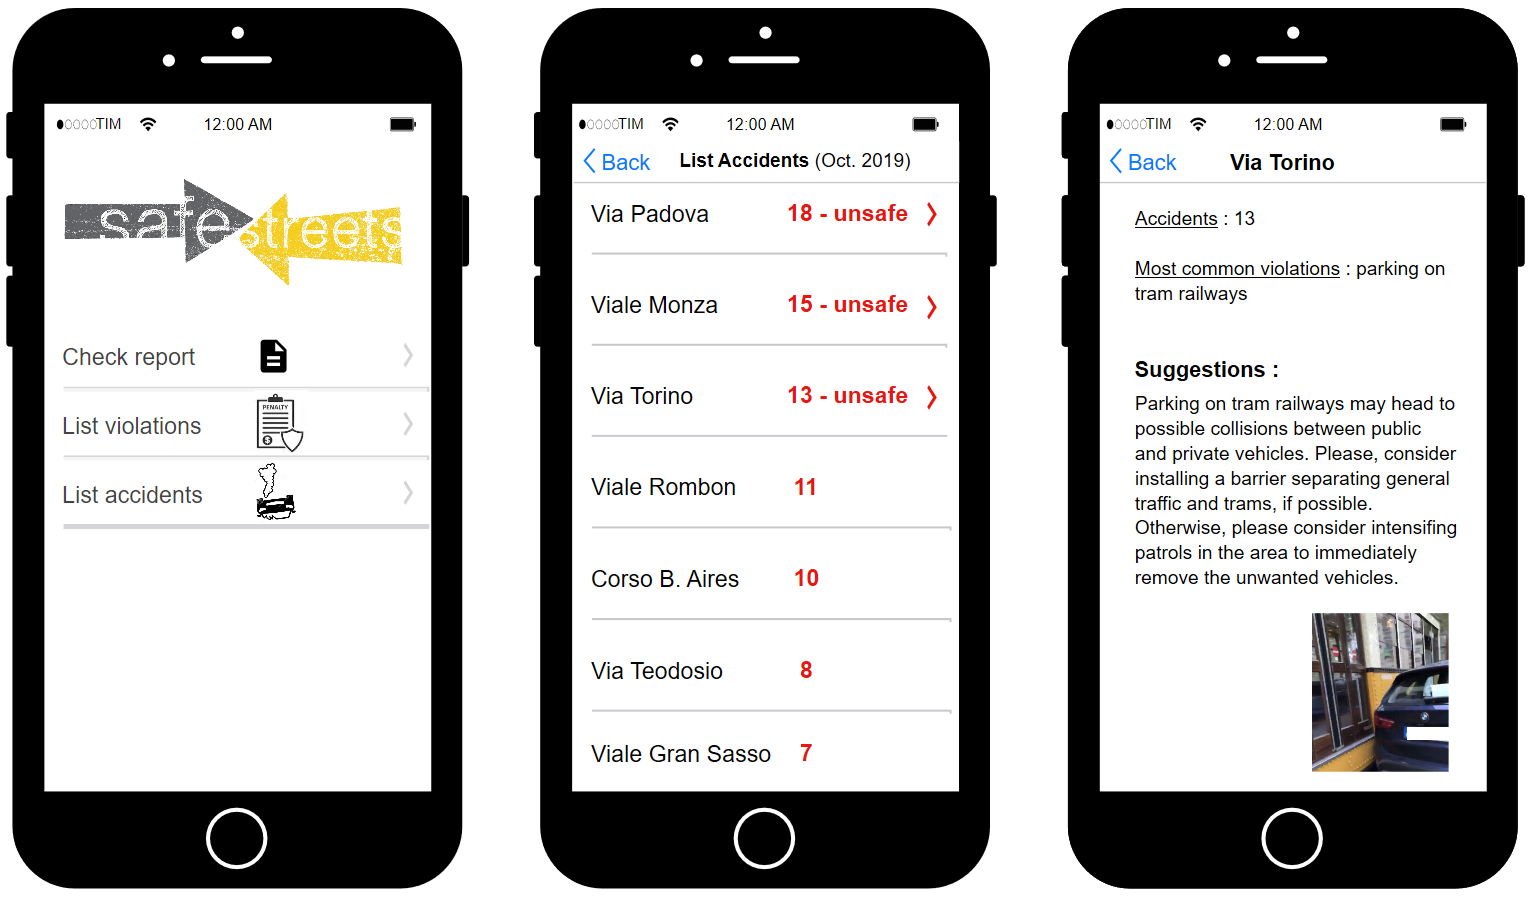
\includegraphics[scale=0.48]{Images/Templates/Authority/auth_0.PNG}
\caption{\label{fig:Mockup-4}Menu and List Accidents section}
\end{figure}

Authorities can select unsafe streets from the section regarding accidents. If said street is listed as \textit{unsafe}, the type of most common violations is shown. A suggestion is made accordingly, as it can be argued that if drivers tend to reiterate a specific mistake, it is possible that this is the cause of the accidents.


\begin{figure}
[H]
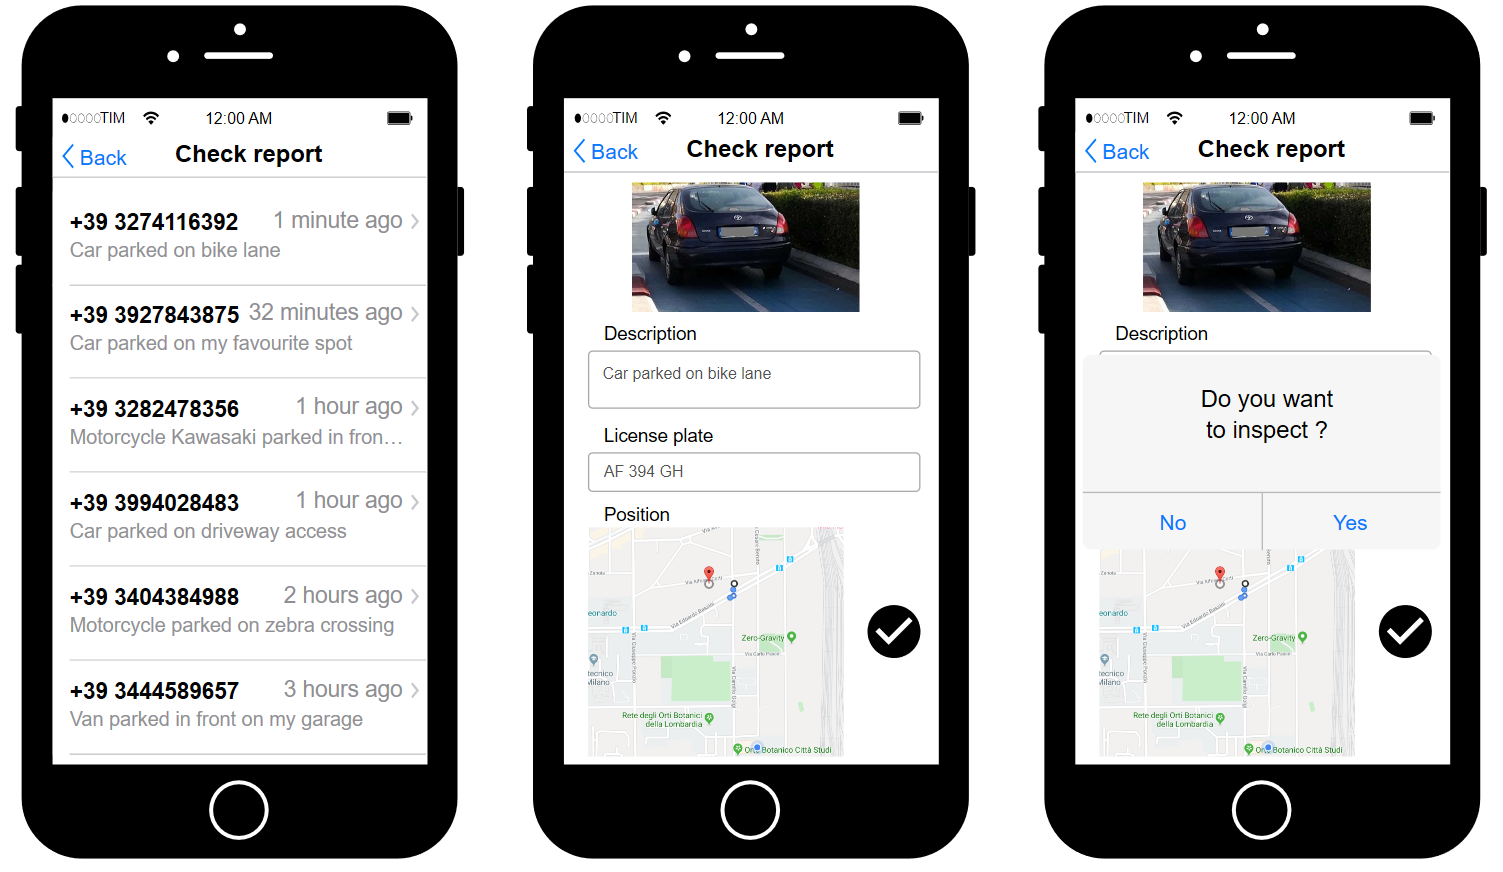
\includegraphics[scale=0.49]{Images/Templates/Authority/auth_1.PNG}
\caption{\label{fig:Mockup-5}Check Report section}
\end{figure}

Authorities can discard specific violations or take them in charge. If the latter happens, they are guided to the site of the violation exploiting GM' API.

\begin{figure}
[H]
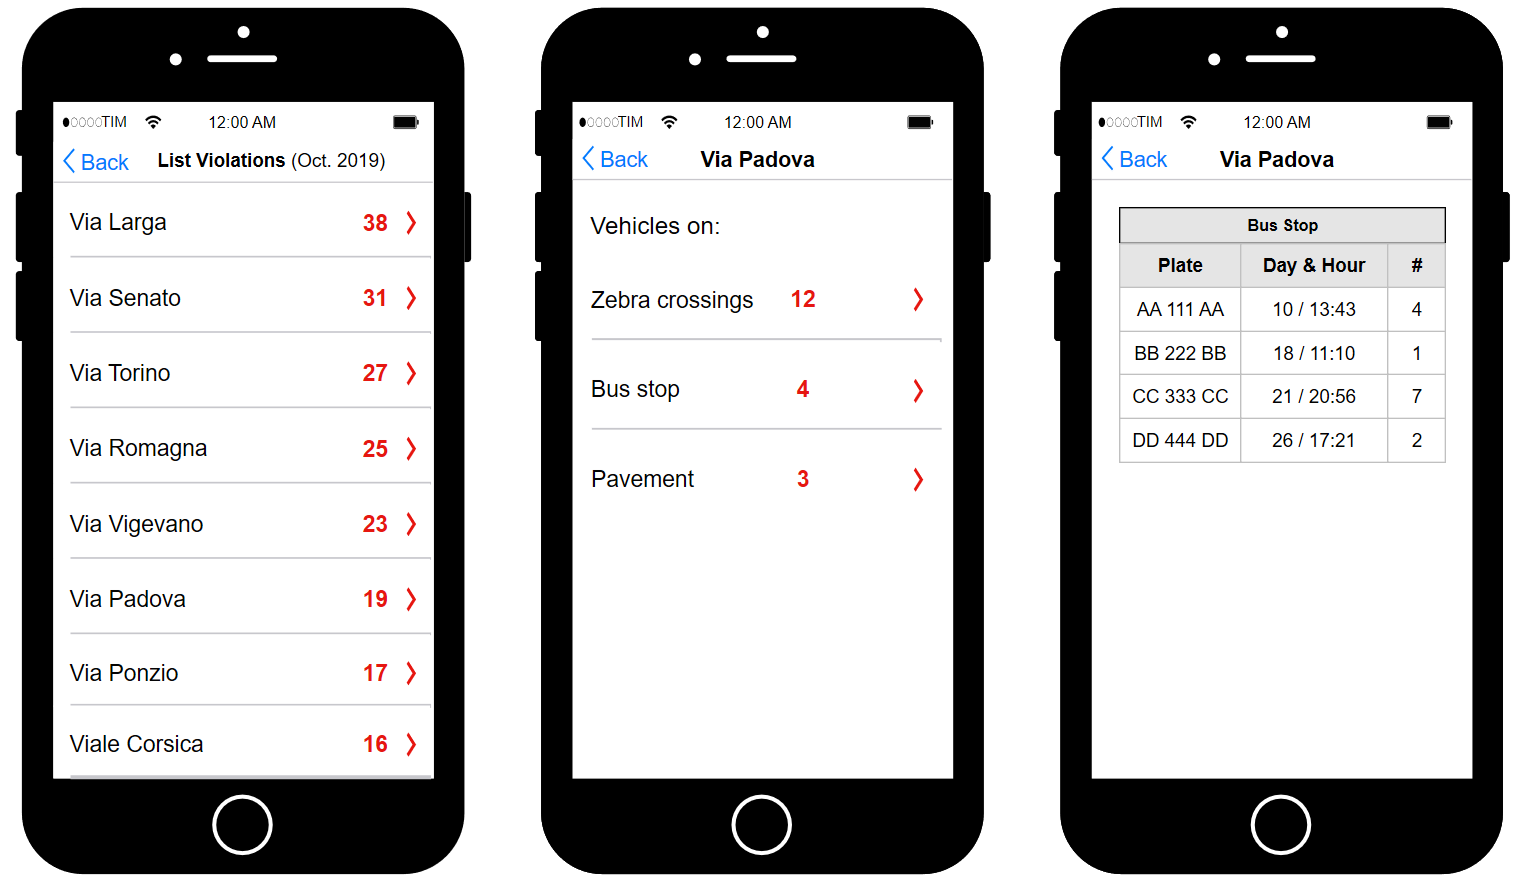
\includegraphics[scale=0.48]{Images/Templates/Authority/auth_2.PNG}
\caption{\label{fig:Mockup-6}List Violations section}
\end{figure}

Authorities can see the list of the offenders, street by street, for any kind of violation.

\begin{figure}
[H]
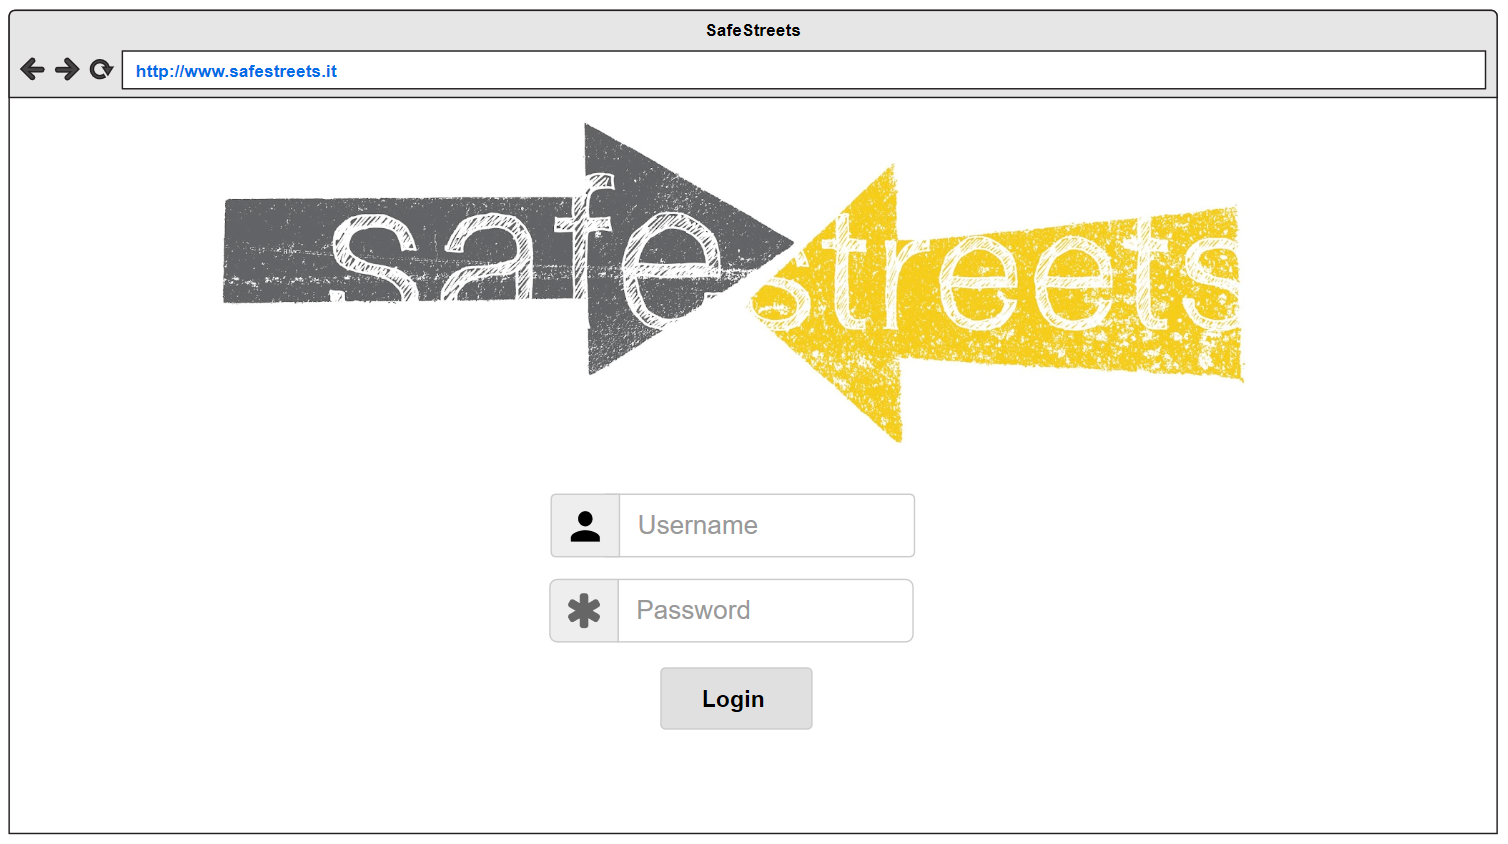
\includegraphics[scale=0.5]{Images/Templates/Authority/auth_3.PNG}
\caption{\label{fig:Mockup-7}Web Login interface}
\end{figure}

Safestreets is provided with a web interface for those authorities who are assigned to administrative section.

\begin{figure}
[H]
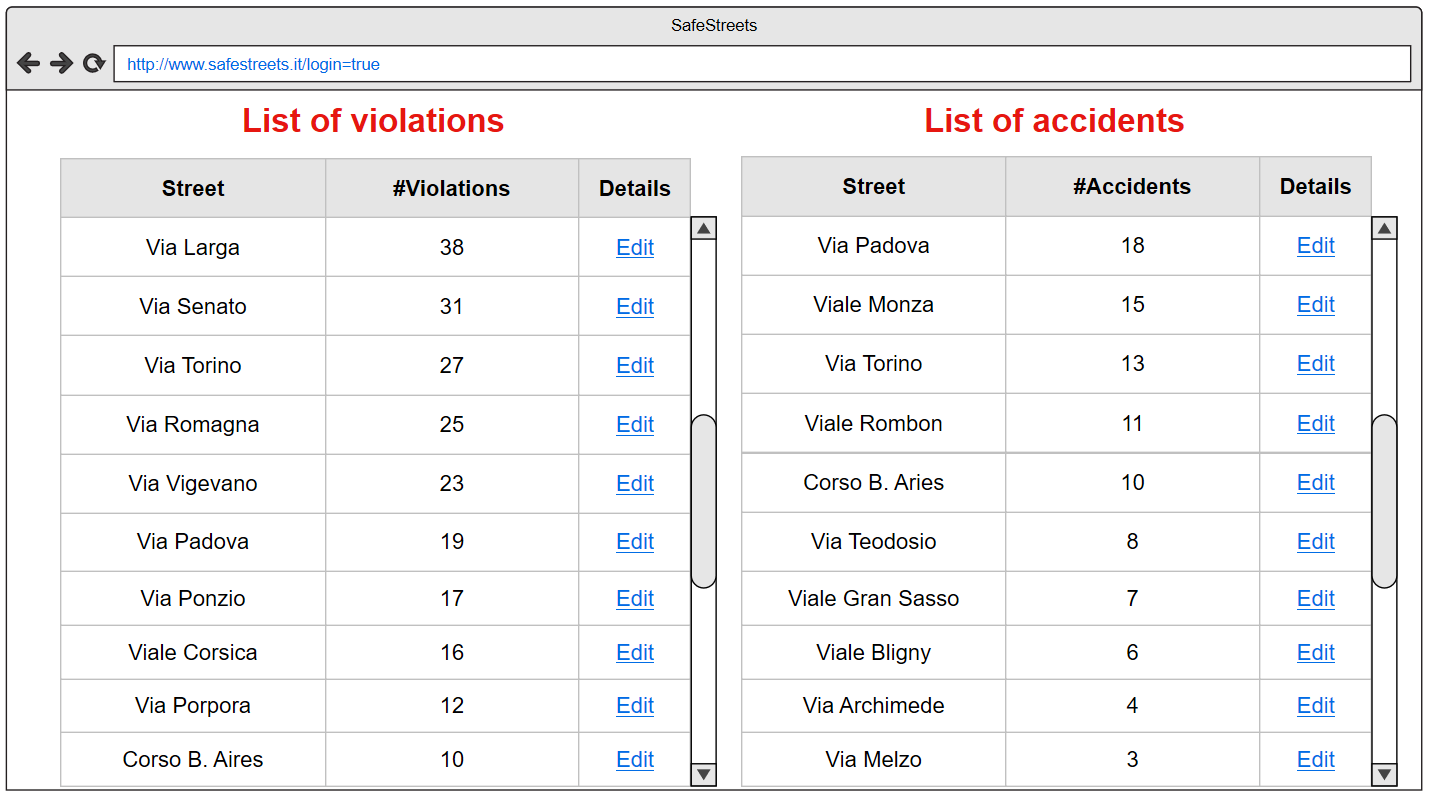
\includegraphics[scale=0.5255]{Images/Templates/Authority/auth_4.PNG}
\caption{\label{fig:Mockup-8}Web interface}
\end{figure}

This version is used merely for data analysis and inspection.

\subsubsection{Hardware Interfaces}

The application is available to those who have a smartphone with internet connection (to communicate with SafeStreet), a camera (to take photos of the violations) and a GPS tracker (to provide the position).
The web application for authorities can be accessed by any computer with a web browser.

\subsubsection{Software Interfaces}

\begin{itemize}

\item Browser
\item Web Server Application
\item Operating System: iOS, Android
\item DBMS

\end{itemize} 

\subsubsection{Communication Interfaces}

This application requires an Internet connection for the purpose of transmitting the report information, HTTPS protocol is used to transfer the data securely between the user and the DBMS.

\subsection{Functional Requirements}
\begin{outline}

\1  \textbf{G1} The application has to store all the information about violations sent to it, until a ticket is either dropped or accepted by an authority

\2 \textbf{D5}: There is no failure in communication

\2 \textbf{D7}: Data storage is reliable

\2 \textbf{R1}: Users must login with their cellphone number to send a violation


%____________________________________________________________________________

\1  \textbf{G2} The system must accepts violations issued from every part of the covered area

\2 \textbf{D1}: The smartphone of the user can provide accurate location

\2 \textbf{D3}: Internet connection is reliable

\2 \textbf{D4}: The CNN is always on and ready to communicate

\2 \textbf{D5}: There is no failure in communication

\2 \textbf{R2}: Users must be connected to the internet with their GPS enabled to use the service

%____________________________________________________________________________

 
\1  \textbf{G3} The system must allow authorities to access violations in every part of the covered area

\2 \textbf{D3}: Internet connection is reliable

\2 \textbf{D5}: There is no failure in communication

\2 \textbf{D6}: GM is always on and ready to communicate

\2 \textbf{D7}: Data storage is reliable

%____________________________________________________________________________

\1  \textbf{G4} The application allows users and authorities to mine information on the system

\2 \textbf{D3}: Internet connection is reliable

\2 \textbf{D5}: There is no failure in communication

\2 \textbf{D7}: Data storage is reliable

%____________________________________________________________________________

\1  \textbf{G5} The application identifies unsafe areas crossing its informations with those offered by the municipality

\2 \textbf{D7}: Data storage is reliable

\2 \textbf{D8}: Data offered by municipality is correct

\2 \textbf{D9}: Data offered by municipality is up-to-date


%____________________________________________________________________________

\1  \textbf{G6} The application suggests possible solution to problems perceived after the crossing of information

\2 \textbf{D2}: The data provided by the user is correct

\2 \textbf{D8}: Data offered by municipality is correct

\2 \textbf{D9}: Data offered by municipality is up-to-date

\end{outline}

\subsubsection{Use Case Diagrams}
\begin{figure}
[H]
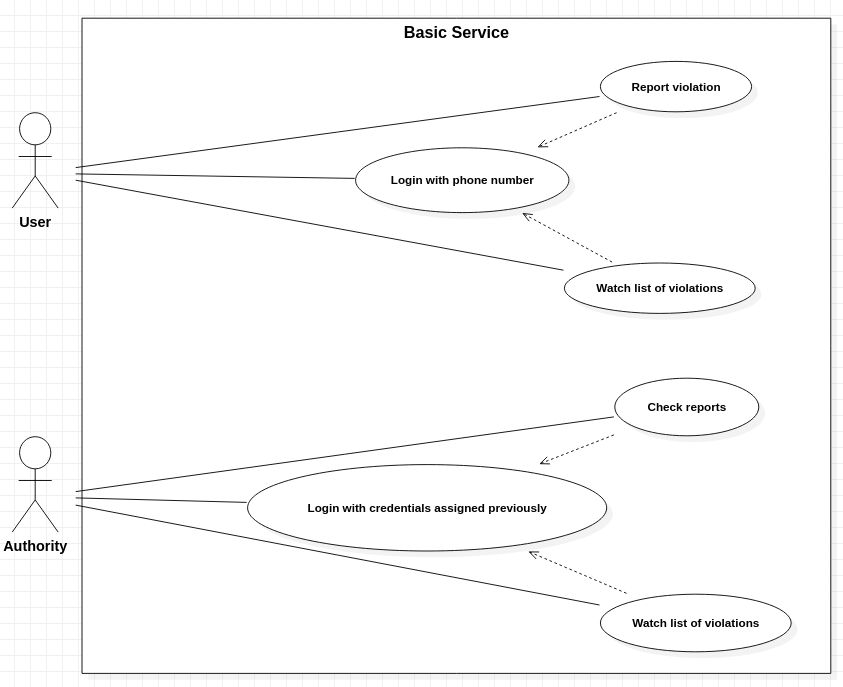
\includegraphics[width=\textwidth]{Images/Diagrams/UseCase1.png}
\caption{\label{fig:UseCase1}SafeStreets basic service use case diagram}

\end{figure}

\begin{figure}
[H]
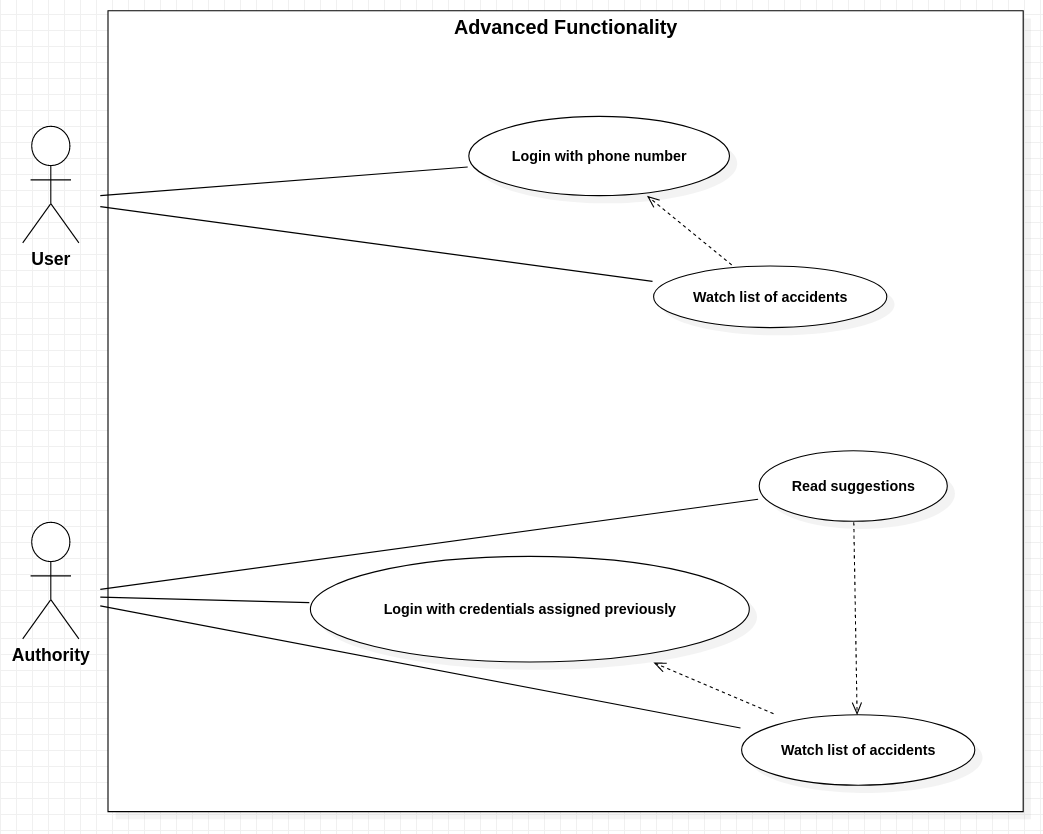
\includegraphics[width=\textwidth]{Images/Diagrams/UseCase2.png}
\caption{\label{fig:UseCase2}SafeStreets advanced functionality use case diagram}
\end{figure}

\subsubsection{Use Case Templates}

\subsubsection{Sequence Diagram}
\begin{figure}
[H]
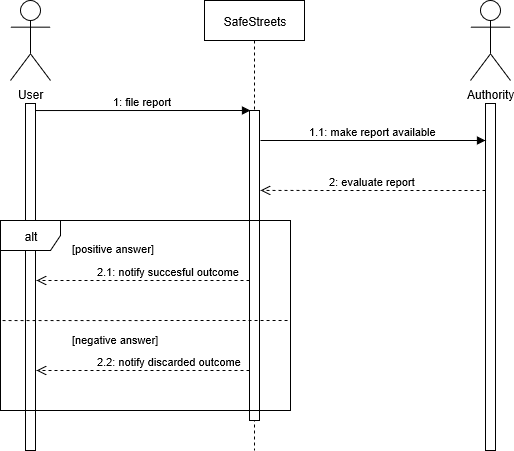
\includegraphics[width=\textwidth]{Images/Diagrams/Sequence1.png}
\caption{\label{fig:Sequence1}Lifetime of a report}
\end{figure}

\begin{figure}
[H]
\centering
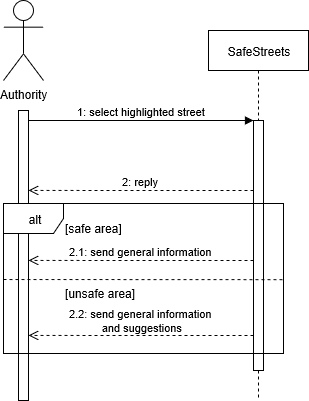
\includegraphics[scale=1]{Images/Diagrams/Sequence2.png}
\caption{\label{fig:Sequence2}Examination of accidents}
\end{figure}